
\documentclass{ar-1col}

\usepackage{amsmath}
\usepackage[comma]{natbib}
\usepackage{url}
\setcounter{secnumdepth}{4}

% Metadata Information
\jname{Xxxx. Xxx. Xxx. Xxx.}
\jvol{AA}
\jyear{2020}
\doi{10.1146/((please add article doi))}



\begin{document}

% Page header
\markboth{Hassan and Zhang}{The Economics of Currency Risk}

% Title
\title{Title: Subtitle}


% Authors, affiliations address.
\author{Tarek A. Hassan,$^1$ and Tony Zhang$^2$ \affil{$^1$Department of Economics, Boston University, Boston, USA, 02213; email: thassan@bu.edu} \affil{$^2$Board of Governors of the Federal Reserve System, Washington, USA, 20551; email: tony.zhang@frb.gov}}



\title{The Economics of Currency Risk\thanks{}}



\begin{abstract}
  This article reviews the literature on currency risk with a focus on its macroeconomic origins and implications. A growing body of evidence shows that countries with safer currencies enjoy persistently lower interest rates, a lower required return to capital, and accumulate relatively more capital than countries international investors perceive as risky. While earlier research has focused mainly on the role of currency risk in generating violations of uncovered interest parity and other financial anomalies, more recent evidence also points to important implications for the allocation of capital across countries, the efficacy of exchange rate stabilization policies, the sustainability of trade deficits, and the spill-over of shocks across borders.
\end{abstract}


% Keywords, etc.
\begin{keywords}
  keywords, separated by comma, no full stop, lowercase
\end{keywords}
\maketitle

% Table of Contents
% \tableofcontents

\section{Introduction}


A key tenet in economics is that the degree to which firms should be willing to invest in a given project depends crucially on the required rate of return to capital: A price-taking firm should install just enough capital so that its marginal product of capital, $MPK_i$, equals the required rate of return to capital, $r_i$,
\begin{equation}
  MPK_i=\underbrace{r^f+RP_i}_{r_i}.
  \label{eq_one}
\end{equation} 
This equation is the point of departure for many classic questions in economics. Students of asset pricing are taught that a firm's $r_i$ has two components; a risk-free part, $r^f$, and a risk-premium, $RP_i$, that depends on the firm's risk characteristics. One of the classic puzzles in asset pricing asks why $RP_i$ is so large relative to $r^f$ (the equity premium puzzle). Monetary economists are interested in the Federal Reserve's power to increase or decrease investment by manipulating $r^f$, while students of economic growth often take differences in $MPK_i$ as a measure of inefficiencies in the allocation of capital across countries, sectors, and firms.

In this article we argue that recent insights from the study of currency risk premia have important lessons for how we should think about Equation \eqref{eq_one}, and by extension, for its key applications in asset pricing, macroeconomics, and economic growth. The simplest, and perhaps and most important, of these lessons is that countries differ dramatically in their risk-free interest rates. These differences in risk-free interest rates are large (on the same order of magnitude as the equity premium puzzle), appear to be highly persistent over time (lasting for decades rather than years), and cannot be explained by predictable depreciations, government default, or differences in inflation rates. Instead, these differences in interest rates appear intimately linked to the risk characteristics of the country's exchange rate, and to its exchange rate regime.

\begin{figure}
  \centering
  \caption{Risk-free Interest Rates}
  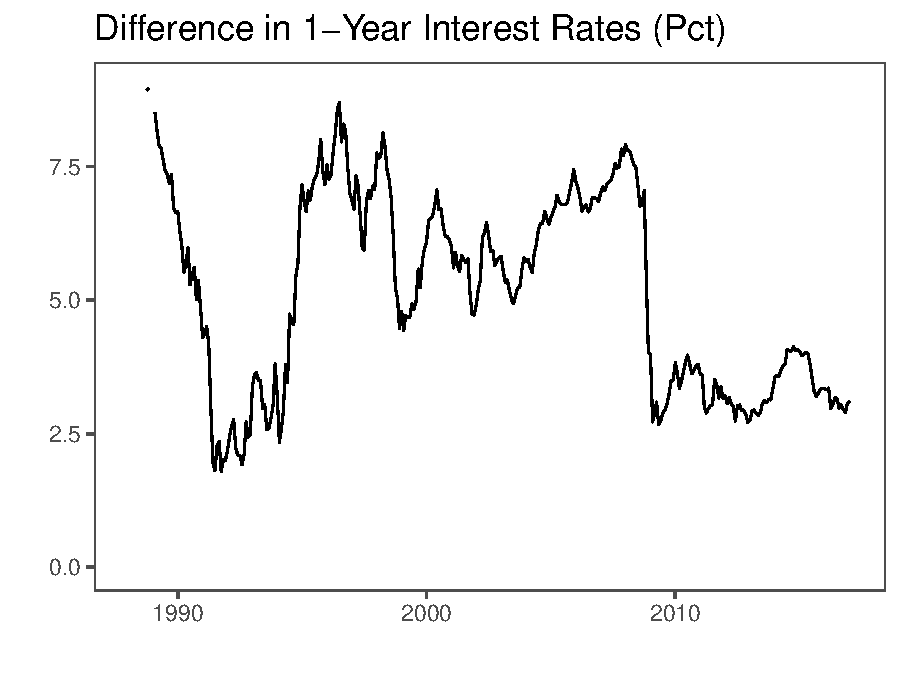
\includegraphics[width=0.7\textwidth]{Exhibits/Figure_FP12M_DiffJPYNZD.pdf}
  \label{fig:fp}
\end{figure}
Figure \ref{fig:fp} shows the difference in the risk-free interest rates of the New Zealand Dollar and the Japanese Yen as an example (we will discuss below how one can measure such risk-free rates and compare them across countries). The figure shows that the New Zealand dollar had a higher risk-free rate than the Japanese Yen in \textit{every} month between January 1988 and December 2016. On average, this difference was about 5.26pp on an annualized basis. When we adjust for movements in exchange rates over the period, the difference in returns on the two countries currencies is 5.10pp -- meaning that a US investors who borrowed in Yen and lent in New Zealand Dollars on average made a return of 148 percent over this period. (For comparison, the equity premium on US stocks was about 7.95pp during the same period.)

We now know that such highly persistent differences in interest rates, similar to those between New Zealand and Japan, are common in the data, even among developed economies. These large differences in interest rates do not appear to be equalizing over time and translate into large differences in returns investors can earn when investing in these currencies.

Why would $r^f$ differ permanently across countries? The emerging consensus in the literature is that the most likely explanation are currency risk premia -- the idea that some currencies are safer investments than others.

A useful way of thinking about this problem is to take the perspective of a retail investor in a third country, say in Hong Kong. As is common in many countries, Hong Kong-based banks regularly offer savings accounts denominated in multiple currencies, so that our fictitious investor might have the option to invest in yen at a deposit rate of 0.1\% or in New Zealand Dollars at a rate of 3.0\%. How might she decide between these two options? Since both accounts are with the same bank, any likelihood of sovereign default is irrelevant. Similarly, our Hong-Kong based investor does not care about inflation in these two faraway countries. Instead, the only relevant factors for her choice between these two investment is the difference in interest rates and the stochastic behavior of the yen-to New Zealand dollar exchange rate.

Because changes in exchange rates are largely unpredictable over short horizons, our investor should not expect either currency to depreciate over the coming year, leaving only one relevant consideration: covariance.\footnote{A regression of the log change in the Japanese Yen to New Zealand Dollar exchange rate on their interest rate differential yields an R-squared of 0.08.} Which of the two currencies does our investor trust to retain value in a possible recession or crisis? Intuitively, she might think that Japanese yen are a safer bet -- and she would be right.

Along with a number of other so called ``safe-haven currencies,'' the Japanese yen tends to appreciate relative to the New Zealand dollar during large international recessions and crises.
\begin{figure}[htp!]
  \centering
  \caption{New Zealand Dollar - Japanese Yen Exchange Rate}
  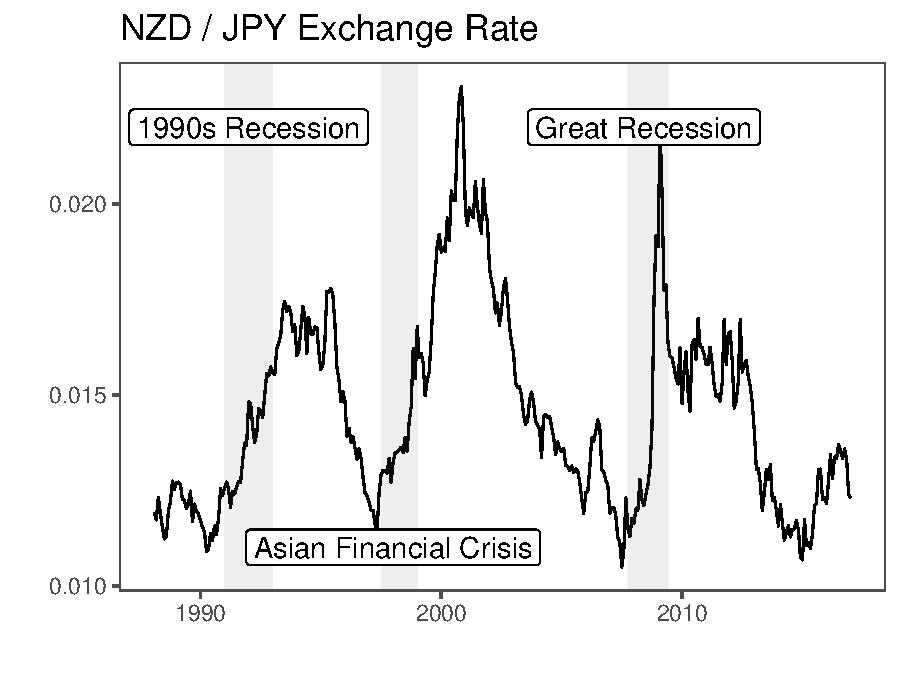
\includegraphics[width=0.7\textwidth]{Exhibits/Figure_FX_JPYNZD.pdf}
  \label{fig:spot}
\end{figure}
Figure \ref{fig:spot} shows some evidence of this pattern by plotting the New Zealand dollar - Japanese yen exchange rate in terms of dollars per yen (so that an increase in the exchange rate indicates yen appreciation). The shaded areas highlight three distinct periods of global economic turmoil: The early 1990s recession (1990 - 1993), the Asian financial crisis (1997 - 1998), and the Great Recession (2007 - 2009). In each of these periods, the yen appreciated markedly against the New Zealand Dollar. If these appreciations during periods of economic turmoil are part of a broader pattern, investors should naturally consider the Japanese yen the safer currency -- and if yen are a safer store of value, it might make sense to accept a lower deposit rate. That is, international investors might be willing to lend at lower rates in currencies they expect to retain value when times are bad.

As it turns out, this simple intuition has a lot of support in the data from international bond and derivatives markets. For example, a seminal paper by \citet{LustigVerdelhan2007} shows that currencies with low interest rates tend to appreciate when US consumption growth is low, and depreciate when US consumption growth is high. That is, there is direct evidence that currencies with low interest rates appreciate when times are bad for US consumers, making these currencies a safer store of value for investors.

In addition to this empirical evidence, the theoretical work on currency risk has identified a number of theoretical reasons to expect the emergence of safe-haven currencies and long-lasting differences in interest rates. In a nutshell, persistent differences in countries' currency risk premia arise naturally in a wide range of international macro models. For example, \citet{Hassan2013} shows that simply allowing for some economies to be larger than others within a standard international real business cycle model is sufficient to generate long-term differences in interest rates between countries, because the currencies of larger countries tend to appreciate when world-wide output is low. That is, even within the most canonical, frictionless, international macro models currency risk premia tend to arise naturally in equilibrium. Other authors have similarly pointed to the emergence of currency premia in models with intermediary capital constraints, trade costs, and differences in resource endowments, among others.

We survey the rapidly growing empirical and theoretical literature on currency risk premia in detail in sections XX and XX. Because the initial focus of this literature was mainly on resolving asset pricing anomalies, many of its key papers tend to use technical finance language. For this reason we attempt to keep this review as non-technical as possible, focusing as much as possible on the underlying economics.

A major difficulty this literature shares with a broader literature in asset pricing is that models with conventional preferences tend to produce risk premia that are quantitatively small. That is, although a number of papers have identified compelling reasons why, for example, the interest rate in Japan should be lower than that in New Zealand, most of these models suggest that it should be lower by something on the order of 0.05pp rather than the 5.26pp we measure in the data. In this sense, the literature is running into a quantitative ``interest differential puzzle,'' which is in some ways analogous to the equity premium puzzle. Both puzzles fundamentally struggle with the prediction of models with standard preferences that risk premia should be small given the relatively small aggregate variation in consumption growth we measure in the data. Quantitative research on currency risk is thus a major area for future research.

Although the literature on currency risk premia has proliferated in recent years, it has perhaps been less successful at making clear the relevance of its findings beyond the financial context, a gap we hope to partially fill with this article.

Perhaps the most immediate implication of currency premia for the real economy is for capital accumulation: If countries differ persistently in $r^f$, then those with higher interest rates have a persistently higher cost of capital and thus, according to equation (\ref{eq_one}) should produce with relatively less capital. Returning to our example from Figure \ref{fig:fp}, it turns out that indeed the capital-to-output ratio in New Zealand is 22 percent lower than in Japan, suggesting that, indeed, the marginal product of capital is larger in New Zealand than it is in Japan. More generally, countries with persistently higher interest rates appear to have higher marginal products of capital in the long-run. This simple insight has direct implications for several strands of literature in macroeconomics, asset pricing, international finance, and monetary economics that have yet to be explored systematically.

The first is for the so-called Lucas-puzzle \citep{Lucas1990}, which posits that, over long periods of time, capital-to-output ratios do not appear to be equalizing across countries, and in particular, not enough capital appears to be flowing to developing nations to equalize the marginal product of capital. If indeed some currencies are permanently riskier than others, then currency risk is one possible factor preventing such equalization. Monetary and fiscal policies that reduce the perceived riskiness of a given currency could then also contribute to equalizing the marginal product of capital across countries. In addition, some of our own recent work suggests that attracting investment by making ones currency a safer store of value for international investors may be a powerful motive determining the choice of a country's exchange rate regime \citetp{HassanMertensZhang2020}.

A second, related, implication is for a large literature that focuses on assessing the efficiency of the allocation of capital across countries \citep{HallJones1997, CaselliFeyrer2007}. A basic assumption in this literature is that $r^f$ is equalized across countries, so that systematic deviations from this required rates can (partially) be attributed to inefficiencies. However, if there are fundamental (efficient) reasons for $r^f$ to differ due to differing currency (and country) risk characteristics, some of these calculations will have to be revisited -- possibly altering our assessment of how much of the discrepancies in income per capita across countries are to blame on inefficiencies.

Third, an active literature in international finance has studied the propensity of firms and countries to borrow in foreign currency \citep{DuSchreger2016, KalemliOzcanetal2019}. If lending in a low-interest-rate currency is safer than lending in a high-interest-rate currency, then the opposite is true for borrowing. That is, firms that borrow in dollar, yen or another safe-haven currency may be loading up on systematic risk -- a price they pay for enjoying lower rates. This systematic risk may then be a concern threatening the resiliency of firms balance sheets and governments' solvency during major crises.

Fourth, long-lasting differences in interest rates across countries may also change how we think about the sustainability of trade and current account deficits. For example, the sustainability of the US current account deficit depends crucially on its ability to borrow cheaply in international markets \citep{GourinchasRey2007}. If there are fundamental economic reasons why the US dollar is a safer currency than many others, then lower US interest rates are here to stay, potentially enabling the United States to sustain trade and current account deficits in perpetuity.

Fifth, time variation in currency and country risk may be one reason for volatile capital flows in and out of emerging markets and the spread of financial and other crises across borders (Miranda-Agrippina and Rey FIXME).

In the remainder of this paper .... FIXMETH


\section{Failures of
  Uncovered Interest Parity and Currency Trades}

Early work on currency risk began as an attempt to understand three puzzling empirical facts in currency markets. The first, often referred to as the \textit{forward premium puzzle}, is that regressions of changes in the exchange rates on differences in interest rates yield a coefficient smaller than one, suggesting that, on average, high-interest-rate currencies do not depreciate enough to wipe out any differences in interest rates \citep{Bilson1981, Fama1984}. The second is that investors in the \textit{carry trade} appear to be making money by borrowing in currencies with low interest rates and lending in currencies with high interest rates. The third puzzling fact is that differences in interest rates and currency returns are highly persistent, so that the same countries tend to have high or low interest rates on a very long-term basis.



\begin{textbox}[h]\section{Measuring Risk-free Interest Rates and Currency Returns}
 In the United States we often regard T-Bills as risk-free. However, even if we assume the US government cannot default, yields on government debt of many other countries are almost certainly contaminated with the possibility of government default.

    For this reason, most of the recent literature constructs synthetic risk-free rates using currency forward contracts and the Covered Interest Parity (CIP) \citep{LustigRoussanovVerdelhan2011, DuSchreger2016}.\footnote{A forward contract is a rate at which a bank agrees to exchange one currency for another at a pre-specified date in the future.} To understand CIP, consider again our example of Japan and New Zealand, and suppose there is a risk-free savings account in each country. A Japanese investor with access to both these accounts and to currency forward contracts then has two ways of making a risk-free investment in yen. First, she can simply save at the yen deposit rate. Alternatively, she can convert yen into New Zealand dollars at the spot exchange rate, invest the New Zealand dollars at the local savings rate, and sign a forward contract to exchange her New Zealand dollars back to yen at the end of her investment period. Both strategies are risk-free since the spot and forward exchange rates are known today. Therefore, if there is no arbitrage, the two strategies must yield the same return:
    \begin{equation}
    \underbrace{1 + r_{JPY}}_{\text{yen risk-free rate}}
    = \underbrace{
        (1 + r_{NZD}) \times \frac{S}{F}
    }_{\text{Implied yen risk-free rate}}.
    \end{equation}
    Taking logs on both sides of this equation and rearranging shows $r_{JPY}-r_{NZD}=s-f$ --- The difference in risk-free interest rates must equal the difference between the (log) spot and forward exchange rates. This difference is known as the forward premium. As a result, we can reliably measure risk-free interest rate differentials from forward prices, even if a given government's ability to repay its debts may be in question.\footnote{For this reason, commercial providers of the carry trade also tend to implement it by buying and selling forward contracts, rather than by trading corporate or government bonds.}.
\end{textbox}

All three of these facts have in common that they describe different violations of uncovered interest parity (UIP), that is, for a given pair of currencies $h$ and $f$, the expected rate of depreciation is usually not equal to the interest differential, $$E\Delta s \neq r^f_h-r^f_f .$$ An extensive literature has documented these violations of UIP and a number of related trading strategies and related facts. \citet{Hodrick1987}, \citet{FrootThaler1990}, \citet{Engel1996}, \citet{Lewis2011}, and \citet{Engel2014} provide excellent surveys.

One difficulty for students of this literature is that it evolved simultaneously as an attempt to understand exchange rate dynamics (e.g. the forward premium puzzle) and asset pricing anomalies (e.g. the carry trade), and thus often alternates between regression-based and portfolio-methods that are not necessarily directly comparable to each other. We next give a brief overview using the unified approach by \citet{HassanMano2019}. This approach allows us to show the main empirical facts in a form where regressions map one-for-one into portfolios, although it also forces us to abstract from many of the details uncovered in the two branches of the literature.

Following this approach, we can implement the carry trade by forming a portfolio at the beginning of each month where we weight each currency by the difference between its risk-free rate, $r^f_{it}$ and the average risk-free rate of all currencies at the time, $\bar{r}_t$. That is, we go long currencies with high interest rates and short currencies with low interest rates, so that we are long and short the same number of dollars. The return on this portfolio is:
\begin{equation}
  \label{eq_carry}
  \textstyle\sum_{i}\left[ rx_{i,t+1}\left( r^f_{it}-\overline{r}^f_{t}\right) \right] ,
\end{equation}%
where, $rx_{i,t+1}=r^f_i-r^f_{USD}+\Delta s$ is the return to borrowing in the home currency and lending in foreign currency $i$ at between $t$ and $t+1$.

Implementing this strategy for 39 currencies between 1986 and 2010 yields an annualized mean return of 5.45 percent with a Sharpe Ratio of 0.54. For comparison, the Sharpe ratio of the U.S. equity market during the same time period is 0.42. The carry trade is therefore highly profitable trading strategy that rivals the equity premium and demands an explanation: are carry traders being compensated for taking on risk? If so, what kind of risk are they taking?

We get the third fact mentioned above from decomposing these returns to the carry trade into a static and a dynamic component. Because interest rates do not change much over time, there is not much benefit from re-sorting the carry trade portfolio every month: on average, our carry trader would have still brought home 70\% of the same returns if she had used only three years of data on interest rates at the beginning of the sample to learn which currencies on average have high and low interest rates, sorted her portfolio once, and then never changed it afterwards.

In fact, \citet{HassanMano2019} show the incremental gain to re-sorting the carry trade portfolio every month is usually not statistically distinguishable from zero. To see how one could assess which variations in currency returns are statistically different from zero, note the carry trade return in (\ref{eq_carry}) is simply the covariance between currency returns at $t+1$ and interest differentials at time $t$. Thus, we can re-write the return to the carry trade as a predictive regression of the form:
\begin{equation}
    rx_{i,t+1} - \overline{rx}_{t+1} 
    = \beta^{ct}\left( r^f_{it}-\overline{r}^f_{t}\right) +\epsilon_{i,t+1}^{ct},  \label{eq_ct}
\end{equation} 
where $\beta ^{ct}$ can be interpreted as the elasticity of expected currency returns with respect to interest rate differentials conditional on a time fixed effect. In our sample of 39 currencies, we estimate $\hat{\beta}^{ct}=0.67 (s.e.=0.16)$. Hence, currencies that have high interest rates compared to other currencies at the same time pay significantly higher returns.

The results from estimating equation \eqref{eq_ct} also imply that for every dollar carry traders make on interest differentials, 1-0.67=0.33 dollars are wiped out by predictable depreciations. In other words, high-interest-rate currencies depreciate on average, but not by enough to eliminate the interest differential.

We should note that there has been some confusion in the literature on this point. In many older papers, authors show regressions of exchange rates on interest rate differentials with a country-specific intercept:
\begin{equation}
    \Delta s_{i,t+1} 
    = \alpha_i + \gamma \left(r^f_{i, t} - r^f_{US, t}\right) + \nu_{i, t+1},
\label{eq_fama} 
\end{equation}
and interpret the fact that the slope coefficient $\gamma$ is often negative as evidence that investors expect high-interest-rate currencies to appreciate instead of depreciate. This finding has prompted a considerable theoretical literature trying to rationalize extremely volatile currency risk premia that are negatively correlated with predicted depreciations (the ``Fama conditions'', \citet{Backusetal2001}). However, this interpretation is incorrect, because a regression with currency fixed effects, such as equation \eqref{eq_fama} is not predictive -- investors at time $t$ do not know what each currency's fixed effect is. \citet{HassanMano2019} show that once one corrects for this discrepancy between realized and predicted appreciations, one recovers results consistent withe the view that, on average, investors expect high-interest-rate currencies to depreciate, not appreciate. This finding of course does not preclude the possibility that investors may expect or may have expected some high-interest-rate currencies to appreciate in specific historical circumstances. That is, the Fama conditions may be relevant in specific instances, but they do not describe the typical behavior of a typical currency in the post Bretton-Woods era.

To summarize, the carry trade is highly profitable because there are highly persistent differences in risk-free interest rates across currencies that are only partially, but not fully, reversed by predictable depreciations. Currencies with higher interest rates on average pay higher returns to international investors than currencies with lower interest rates. Taken together, these three stylized facts form the empirical basis for the notion that there may be long-lasting differences in the risk characteristics of different currencies.

In addition to these major stylized facts, researchers have also documented a number of additional patterns in violations of UIP that have so far received relatively less attention by theorists. \citet{ChinnMeredith2004} looked at long-term bonds and find that UIP tends to hold at longer maturities. In other words, the currency of the high-interest-rate country tends to depreciate in the long-run to negate differences in interest rates. In related work, \citet{LustigStathopoulosVerdelhan2019} show that the returns to currency carry trades also decrease with the maturity of the bonds. \citet{LRV2014} show another highly profitable trading strategy is the dollar carry trade: A trade where investors buy non-U.S. currencies whenever the average interest rate amongst advanced economies is higher than that of the U.S. \citet{LustigRichmond2020} show that currencies of countries that are farther away from all other countries are riskier currencies.


\section{Interest Rate Differentials as Differences in Risk Premia}

\subsection{Reduced-form Evidence}

To formally attribute the returns of currency traders to risk, we borrow some technology from the broader asset pricing literature. The classic empirical asset pricing literature constructs \emph{risk-factors} to attribute cross-sectional differences in asset returns to different sources of risk by looking for comovement in asset returns \citep{Fama1976}. Typically, researchers sort assets based on some characteristic of interest, and then divide assets into a small number of portfolios based on the sort. The first portfolio typically contains assets with the lowest values of the characteristic of interest, and the last portfolio typically contains assets with the highest values. A risk factor is then constructed by taking the difference in returns between the fist and last portfolio. Researchers determine a risk factor explains asset returns by running regressions of returns on the risk factor, and showing that assets with higher regression coefficients (``loadings'') on the risk factor also obtain higher expected returns.\footnote{For example, \citet{FamaFrench1992} constructed two risk factors by sorting U.S. equities into portfolios based on market capitalization and book-to-market ratio, and showed portfolios of stocks with greater exposure to these two risk factors obtained higher average returns.}

% A key innovation of the empirical asset pricing literature is also to analyze portfolio returns rather returns than on individual assets. Again, assets are sorted into portfolios based on some dimension of interest. Intuitively, averaging the returns of assets within portfolios eliminates diversifiable and asset-specific risks. The remaining variation in returns across portfolios should better capture the risk-return trade-off specifically from differing along the dimension of interest.

In a seminal paper, \citet{LustigRoussanovVerdelhan2011} applied these techniques to exchange rates and provided systematic evidence that the greater returns obtained from investing in high-interest-rate currencies result from greater risk exposure. For every month between November 1983 and December 2009, the authors sorted currencies into 6 portfolios based on their risk-free rate differential relative to the U.S. dollar. The first portfolio contained currencies with the lowest risk-free rates and the last portfolio contained currencies with the highest risk-free rates. The authors constructed a \emph{carry trade risk factor} by taking the difference in the returns between the portfolio containing the highest-interest-rate currencies and the portfolio containing the lowest-interest-rate currencies.

\citet{LustigRoussanovVerdelhan2011} showed that differential exposure to their carry trade risk factor accounted for cross-sectional variation in the expected returns from investing in different currencies. The authors regressed the currency returns of their currency portfolios on the carry trade risk factor, and showed the portfolios with higher-interest-rate currencies obtained a higher average return and also covaried more positively with the risk factor. An increase in the loading on the carry trade risk factor from 0 to 1 was associated with a highly significant increase in excess returns of 5.5 percent per year.

In this sense, \citet{LustigRoussanovVerdelhan2011} identified a common source of risk in currency markets, and showed that exposure to this common source of risk explained cross-sectional differences in currency returns. However, the major drawback of this asset pricing method is that it does not reveal the ultimate source of risk. In other words, we know exchange rates move with each other, but we do not know the economic forces that drive this comovement.

Many researchers have therefore tried to identify relationships between currency returns and macro-financial variables to understand the sources of currency risk. \citet{LustigVerdelhan2007} showed that low-interest-rate currencies provide a hedge against U.S. consumption growth risk. Low-interest-rate currencies systematically appreciate when U.S. consumption growth is low, and high-interest-rate currencies tend to depreciate when U.S. consumption growth is low. Thus, the U.S. investor can hedge against periods of low consumption growth by investing in a portfolio of low-interest-rate currencies. U.S. investors find this hedging property useful, and, as a result, accept a lower rate of return for investing in low-interest-rate currencies.

Others have highlighted the resiliency of low-interest-rate currencies to periods of financial turmoil. \citet{LustigRoussanovVerdelhan2011} and \citet{CampbellMedeirosViceira2010} both showed low-interest-rate currencies tend to appreciate whenever equity markets are volatile whereas high-interest rate currencies tend to depreciate. Instead of using data from equity markets, \citet{Menkhoffetal2012} measure of periods financial market turmoil using an average realized exchange rate volatility. High-interest-rate currencies tend to depreciate in response to increases in the average realized exchange rate volatility, whereas low-interest-rate currencies tend to appreciate. Thus, low-interest-rate currencies also provide a hedge against global exchange rate volatility. 

Another strand of the literature stresses the presence of crash risk as a main driver of currency excess returns. \citet{Brunnermeieretal2009} studied eight major currencies and showed high-interest-rate currencies exhibited a greater chance of experiencing large devaluations (i.e. crash risk) whereas lower interest rate currencies did not. Jurek2014 formally assesses the share of carry trade returns explained by currency crash risk by constructing carry trades that are protected from crash risk. Specifically, \citet{Jurek2014} invests in a portfolio comprising the carry trade as well as currency options that protect against large exchange rate fluctuations (around 1.4 times the magnitude of the monthly standard deviation). He found that buying protection from crash risk decreased the returns to the carry trade by about a third. Thus, the presence of crash risk explains about a third of the carry trade. Farhietal2015 proposes a structural model of currency returns that are driven by the presence of crash risk. The authors calibrate the model using currency options data and also find that eliminating crash risk would reduce carry trade returns by a third.


% \begin{itemize}
% \item Lewis2011 - peso problems (no risk premia, simply mismeasuring
%   average returns due to small samples)
% \end{itemize}

Ultimately, each of these papers highlight different ways in which high-interest-rate currencies may be riskier than low-interest-rate currencies. However, the common thread among these papers is that persistent differences in the returns to investing in different currencies reflect persistent differences in risk premia. Low-interest-rate currencies provide lower returns to investors because they are safer currencies, and tend to appreciate during periods of economic distress. Meanwhile, high-interest-rate currencies depreciate during periods of economic distress, and must therefore reward investors with higher excess returns.



\subsection{Theory: Microfoundations of Safe Haven Currencies}

Prompted by this empirical evidence, the theoretical literature has identified several fundamental economic forces that may make a given currency safer or riskier from the perspective of global investors. Although there is an ongoing debate on which of these forces may be most important in practice, many of of these microfounded models share a common structure, which we can summarize using just a few key equations.

Consider a world economy in which international assets are priced by the marginal utility of an international investor, $\lambda_T$, which will be our measure of ``good'' and ``bad'' times. Times are good when $\lambda_T$ is low, and times are bad when it is high. In different models, $\lambda_T$ may be the marginal utility of consumption of traded goods (the part of consumption that his shared internationally), the marginal utility of consumption of a key investor who intermediates between segmented international markets, or the capital constraint of such an intermediary. Households consume a country-specific final good, the price of which (accounted for in a common unit) depends on $\lambda_T$ and a country-specific shock, $x^n$,
\begin{equation}
  p^{n} = a\lambda_{T} + b x^{n}.  
  \label{eq_RF}
\end{equation}%
The country-specific shock interchangeably may stem from a country-specific supply, demand, or monetary shock; in other words, it is a stand-in for any factor that affects the price of consumption in one country more than in others. The higher $x^{n}$, the higher the price of domestic consumption relative to that in other countries. For simplicity, assume $\lambda _{T}\sim N(0,\sigma^2_{\lambda_{T}})$ and $x^{n} \sim N(0,\sigma^2_x) $ are normally distributed, not necessarily independent, shocks and $a$ and $b$ are positive constants.

The real exchange rate, $S^{f, h}$ between two countries $f$ and $h$ is the relative price of their respective final goods. In logs,
\begin{equation}
  s^{f,h} 
  = p^f - p^h 
  = b(x^f - x^h),
\label{eq_RER}
\end{equation}
where the second equality substitutes Equation \eqref{eq_RF}. Because of $x^{n}$, the relative price of consumption may differ between the two countries, allowing the real exchange rate to move. When the price of consumption in country $f$ increases, its consumption bundle appreciates relative to country $h$. In this sense, we can speak of ``currencies'' even without formally introducing money into the model.


By definition, the risk-free bond in country $h$ pays $p^h$ with certainty, while that in country $f$ pays $p^f$ with certainty, so that each country's risk-free bond pays exactly one unit of that country's consumption bundle. Importantly, because the real exchange rate may move around, country $h$'s risk-free bond is not risk-free from the perspective of households in country $f$, and vice versa. For this reason, one country's risk-free bond may be more expensive than the other country's risk-free bond. The risk-free rate of interest is the yield to maturity of the risk-free bond, so that the country with the more expensive risk-free bond automatically must have the lower risk-free rate of interest. In this sense, any model with a variable real exchange rate as in equation (\ref{eq_RER}) may produce differences in risk-free interest rates across countries.

Different theories of such differences in interest rates apply elementary asset pricing to equation (\ref{eq_RER}). One can show that the log expected return to borrowing in country $h$ and to lending in country $f$ is
\begin{equation}
  r^{f} + \Delta \mathbb{E} s^{f,h} - r^{h} =cov\left( \lambda _{T},p^{h}-p^{f}\right),
  \label{eq_UIP_RF}
\end{equation}%
where $r^{n}$ is the risk-free interest rate in country $n$.\footnote{$\Delta\mathbb{E}s^{f,h}$ is defined as the logarithm of the ratio of the countries' expected real price changes. See Appendix \ref{Appendix_ReducedFormResults} for a formal derivation.} This statement means a currency that tends to appreciate when $\lambda_T$ is high pays a lower expected return and, if $\Delta \mathbb{E} s^{f,h}\approx0$ (as is the case in the data), therefore must has a lower risk-free interest rate. That is, a currency that appreciates in bad times (for example, in times when consumption goods are expensive everywhere) provides a hedge against worldwide consumption risk and pays lower returns in equilibrium.

Equations \eqref{eq_RF} and \eqref{eq_UIP_RF} are the main ingredients of risk-based models of unconditional differences in interest rates across countries, where different approaches have identified different reasons why the countries differ in the degree to which their price indices covary with $\lambda_T$.

\begin{textbox}[h]
\section{Currency vs. Country Risk}
Although we follow the literature in referring to the spread in (\ref{eq_UIP_RF}) as stemming from ``currency risk,'' it is important to note that equation (\ref{eq_RER}) to (\ref{eq_UIP_RF}), as well as virtually all models written on the subject, describe the stochastic behavior of the real, not the nominal, exchange rate. Fundamentally, what we mean by ``currency risk'' is therefore the risk that comes from country-specific shocks to a country's consumer price index. Different models may invoke various supply, demand, or monetary shocks for this purpose, but most models we shall discuss below actually do this without even formally introducing money into the model. In this sense, it may actually be more accurate to speak of ``country-specific risk'' or ``country risk.'' 
\end{textbox}


\paragraph*{Spillovers: Country Size and Trade Centrality}

Perhaps the most obvious reason for such differences in covariance to arise are differences in how important a given country is for the world economy. In particular, most models of exchange rate determination suggest that any shock that raises the price of consumption in a larger economy will also make the part of consumption that is shared internationally more expensive, so that $\lambda_T$ will tend to rise more in response to a shock that raises the price of consumption in a larger country. That is, larger countries tend to appreciate in high-marginal-utility states, so that their currencies retain value precisely when marginal utility is high in the world. These safer currencies of larger countries then naturally have lower interest rates and pay lower returns to international investors. This is essentially the argument in \citet{Martin2012} and \citet{Hassan2013}.

This result is easiest to see in a frictionless model with traded and non-traded goods, where $\lambda_T$ coincides with the marginal utility of traded consumption, which must then be equalized across countries in equilibrium, and $p^n$ coincides with the marginal utility of overall consumption in country $n$. Whatever country-specific supply, demand, or monetary shock raises a given country's $p^n$ then typically also prompts this country to import more traded goods. While a small country's imports, by definition, have no effect on the world supply of traded goods, rising imports by a large country will make these traded goods relatively scarce in world markets, raising their price, and increasing $\lambda_T$, so that
\begin{equation} \lambda_{T} = -c \sum_{n} \theta^n x^n,
    \label{eqn:lambdat2NP}
\end{equation}
where $\theta^n$ is a measure of country $n$'s share of world GDP. It then follows immediately that larger country's consumption bundles tend to appreciate when $\lambda_T$ is high. Comparing (\ref{eqn:lambdat2NP}) with (\ref{eq_RER}) and (\ref{eq_UIP_RF}) yields
\begin{equation}
  r^{f} + \Delta \mathbb{E} s^{f, h} - r^{h}
  =g\left(\theta^h - \theta^f\right) \sigma_x^2,
  \label{eq_FF_UIP}
\end{equation}
so that larger countries have have lower interest rates, and their currencies are a safer store of value and pay lower returns on average.
  
Variations of this result in \citet{Hassan2013} also show that, by the same logic, firms producing non-traded (that is, country-specific goods) in larger countries should have a lower cost of capital, and that joining a currency union (an area that shares a common monetary shock) may lower interest rates in the participating countries.

\citet{Richmond2019} highlights another force that may make a country's economy more or less important for the world economy: its trade centrality. The idea is that shocks to countries that are located near the center of the network of world trade, such as Singapore and the Netherlands, may have an outsized impact on the production of traded goods -- even if they are small. To arrive at this result, he introduces multiple countries and non-traded goods into a model where traded goods are produced with intermediate inputs and a network of input-output linkages (Long and Plosser, 1983; Acemoglu, Carvalho, Ozdaglar, and Tahbaz-Salehi, 2012). Within this framework, shocks that affect central countries spill over more to the rest of the world, because these countries add a (small) amount of value to a large number of goods produced in the world. Shocks that raise the price of consumption in these central countries have a larger effect on  $\lambda_T$, because they are more disruptive to supply chains around the world. As a consequence, the currencies of central countries are safer and pay lower interest rates than the currencies of peripheral countries.   

This result relies on two key assumptions: First, shocks to the production of traded and non-traded goods are positively correlated within countries, so that the same shocks $x^n$ that increase the price of domestic consumption and lead a country's consumption basket to appreciate, also diminish its capacity to add value to the production of traded goods. Second, these shocks are more correlated across countries the more intensive two countries trade with each other. (There is broad empirical support for both of these assumptions.) \citet{Richmond2019} can then show that $$\lambda_{T} = -c \sum_{n} \theta^n x^n- d\sum_{n} \nu^n x^n,$$ where $d$ is a positive constant and $\nu^n$ is a measure of the country's trade centrality.

\paragraph*{Differences in Stochastic Properties of Consumer Price Indices}

While both spillover-based approaches (size and centrality) put structure on which countries' shocks are more or less important for world-wide price of risk ($\lambda_T$), another set of papers study innate differences in the properties of countries' consumer price indices ($p^n$).

\citet{FarhiGabaix2016} study a model where countries differ in their resilience to rare world-wide disasters. The non-traded goods of resilient countries increase in value whenever a disaster strikes, so that these resilient countries appreciate upon the disaster's impact -- making their currencies a safer store of value. Resilient countries therefore have lower interest rates, though it remains unclear how researchers should distinguish resilient and non-resilient countries in practice.

Maggiori (2013), argues that the relatively low interest rates in the United States may be explained if foreign exporters have relatively more trouble accessing trade credit in large financial crises. In his model, the stochastic discount factor depends on intermediary credit constraints, so that ``bad times'' are when it is difficult to obtain credit (that is, in a financial crisis). If these credit constraints bind relatively more in countries that are less financially developed than the United States, then trade credit needed for shipping goods from the rest of the world to the United States becomes relatively more expensive than trade credit for shipping goods from the United States to the rest of the world in a crisis -- making the US consumption bundle relatively more expensive. He suggests this may be one reason why the US dollar tends to appreciate in extreme crisis periods, making the US dollar a safer store of value for international investors.

\citet{Readyetal2013} note that a number of ``commondity countries,'' such as Norway and Australia, largely export basic commodities, such as coal, oil, and iron ore, but rely much more on imports of finished goods than ``producer countries,'' such as Japan and Germany, who export these goods. In their model, total shipping capacity can only adjust slowly over time. In a boom, when output of traded goods is high, more commodities must be shipped from the commodity countries to the producer countries, and more finished goods in the opposite direction. This increased demand for shipping drives up trade costs disproportionately more in the commodity countries because, in effect, any finished goods they consume must travel further. As a consequence, the price of consumption in commodity countries increases in a boom (when $\lambda_T$ is low) and decreases in a downturn, relative to the price of consumption in producer countries. It follows that, in effect, commodity countries appreciate in ``good times,'' and depreciate in ``bad times.'' With quadratic shipping costs we have
\begin{equation*}
  p^{\text{Commodity Country}}-p^{\text{Producer Country}}\sim\left(\frac{\text{Finished goods shipped}}{\text{Shipping Capacity}}\right)^2
\end{equation*}
Additional implications of this model is that the real exchange rates of commodity countries are positively correlated with world-wide commodity prices. 

Powers (2015) derives similar results without appealing to stochastic trade costs, but instead argues that commodity booms drive up wages in commodity countries, so that local non-traded goods become more expensive through a type of Balassa-Samuleson-type labor-cost effect. The consumption bundles of commodity exporters therefore tend to appreciate in world-wide booms and depreciate in world-wide busts, making their currencies riskier than those of non-commodity-exporting countries.

Aside from commodity producing countries, Wiriadinata (2020) points out that countries that have a large amount of outstanding dollar-denominated external debt tend to depreciate whenever the dollar appreciates and have high interest rates and currency returns. She rationalizes this pattern with wealth effect: when the US dollar appreciates, the real value of dollar-denominated debt increases, effectively making countries that borrow in dollars poorer. This negative wealth shock in turn reduces domestic demand, lowering the relative price of domestic non-traded goods, and thus depreciating the currencies of countries that borrow heavily in dollars. If the Us dollar appreciates systematically during international crises (as suggested by the literature above), then these currencies a riskier investment for international investors.

FIXMETH To and Tran


\paragraph*{Portfolio Balance Models} The  ``portfolio balance'' approach to understanding currency risk directly models the capital constraints of financial intermediaries engaged in currency trading. \citet{GabaixMaggiori2015} consider a world in which a financier with limited risk-bearing capacity engages in currency trading. This financier holds onto currencies whenever there is an imbalance in the supply and demand for currencies across countries. In equilibrium, the financier must earn positive expected returns on the currencies she holds in her portfolio. Otherwise, she would not employ any of her limited risk-bearing capacity to absorb currency imbalances. \citet{GabaixMaggiori2015} suggest that in practice financiers are holding onto the assets of net debtor countries. As a result, investing in net debt countries' currencies should obtain positive excess returns. 

Liao and Zhang (2020) provide a model in which the stochastic properties of currencies are determined by investor hedging demands. An investor in a net creditor country hedges her exchange rate risk by buying domestic currency in the forward exchange rate market. Financial intermediaries produce currency forward by buying the currency in spot exchange rate markets and trading in bonds. In practice, investors tend to increase their hedging demands during periods of financial turmoil. As investors in net creditor countries increase their hedging demand, their domestic currency appreciates as financial intermediaries buy more currency in the spot market to produce currency forward. As a result, investor hedging demands result in systematic variation in exchange rates that are in line with countries' net foreign asset positions. Net creditor countries' currencies systematically appreciate during periods of financial turmoil, and should thus pay lower returns in equilibrium.

These two models provide rationales for why currencies of net debtor countries pay higher returns than currencies of net creditor countries. Moreover, both models suggest the currencies of net debtor countries systematically depreciate in bad times. \citet{DellaCorteetal2009} provides systematic evidence for these hypothesis in the data. 
 
\begin{textbox}[h]
\section{Foreign Asset Portfolios and the Reserve Currency Paradox} While we have focused our discussion on interest differentials and violations of UIP, most models make additional predictions about the returns on other assets (such as stocks in the traded and non-traded sector), the composition of equilibrium portfolios, and the co-movement of consumption across countries. One common prediction that is shared between all approaches in which financial markets are somewhat close to complete is that countries with low interest rates should also also be net-importers of insurance from the rest of the world. This result is easiest to see when we think about spillovers: The reason large or trade-central countries have low interest rates is because shocks that hit these important countries spill over to the rest of the world, so that they are harder and more expensive to insure against. After all, saying that risk-fee interest rates are lower in the United States than in New Zealand is the same as saying that US risk-free bonds are more expensive than those in New Zealand.

This typically means that the same forces that make a given country's currency relatively safe will also tend to make this country a net-importer of insurance from the world market. Although the link between country risk and net foreign asset portfolios has not been systematically studied in the data, this prediction appears at odds with the US data, which is generally seen as having both low interest rate and being a net exporter of insurance to the rest of the world (US investors tend to hold equity abroad while foreign investors largely hold US safe assets, such as T-bills, \citep{GourinchasRey2007,GourinchasGovillotRey2017}). \cite{Maggiori2013} calls this puzzling pattern in the US data the ``reserve currency paradox.'' Aside from resolving this puzzle for the United States, future research should also explore whether or not the same puzzling pattern extends to the portfolio holdings of other low-interest-rate countries. 

\end{textbox}






\subsection{Reduced-form Evidence}

While many of the theoretical papers surveyed above provide detailed evidence on each of the particular channels making a given currency safer or riskier from the perspective of world investors, the literature currently lacks a comprehensive evaluation of their relative importance. As a first step in this direction, Table \ref{table:rx_char} shows a set of regressions of currency returns for 31 currencies 1998-2016 on variables that, according to various theories, should be associated with lower interest rates and returns. 
\begin{table}[htp]
\begin{center}
\caption{Currency excess returns and characteristics}
\label{table:rx_char}
\vspace{1em}
\begin{tabular}{l c c c c c }
\hline
\hline
 & (1) & (2) & (3) & (4) & (5) \\
\hline
GDP Share               & $-0.50^{**}$ &             &               & $-1.27^{***}$ & $-1.51^{***}$ \\
                        & $(0.25)$     &             &               & $(0.34)$      & $(0.39)$      \\
Trade Centrality              &              & $-0.41^{*}$ &               &               & $0.43$        \\
                        &              & $(0.22)$    &               &               & $(0.26)$      \\
NIIP / GDP              &              &             & $-0.84^{***}$ &               & $-0.85^{***}$ \\
                        &              &             & $(0.25)$      &               & $(0.23)$      \\
FX Allowed Deviation         &              &             &               & $0.20^{***}$  & $0.15^{*}$    \\
                        &              &             &               & $(0.05)$      & $(0.08)$      \\
\hline
Fixed Effects & Time & Time & Time & Time & Time \\
Num. obs.     & 7,517        & 7,517     & 6,177          & 6,488          & 5,186          \\
R$^2$         & 0.27        & 0.27     & 0.32          & 0.28          & 0.33          \\
\hline
\hline
\end{tabular}
\end{center}
\begin{minipage}[htp!]{\textwidth}
\scriptsize
\emph{Notes:} This table presents regressions of currency excess returns on currency area characteristics. GDP Share is a currency area's share of world GDP. Centrality is a currency area's trade centrality taken from \citet{Richmond2019}. NIIP / GDP is a currency area's net international investment position as a share of GDP. FX Allowed Deviation captures each currency's maximum allowable annual exchange rate deviation relative to its target currency according to \citet{ilzetzki2018exchange}. $^{***}p<0.01$, $^{**}p<0.05$, $^*p<0.1$
\end{minipage}
\end{table}

The first three columns show that a one standard deviation increase in a country's size (GDP share), trade centrality, and net foreign asset position are associated with a 0.5, 0.4 and 0.8 percentage point decrease in the returns on the country's currency, respectively. In addition, column 4 shows that currencies that are stabilized relative to the US dollar or the euro (a lower FX Allowed Deviation) also have significantly lower returns. (We will discuss this finding in section XX below.) When we combine all four variables in column 5, trade centrality loses significance, though the coefficient remains almost unchanged.

While these results are suggestive, they are also inadequate. Because interest differentials are highly persistent, all of these regressions rely to some degree on cross-sectional variation for identification, and with fewer than 40 currencies for which we have reliable data, our statistical power for disentangling the effect of multiple variables is highly limited. Moreover, these regressions have no way of accounting for the ease with which each of the candidate mechanisms can account for the numerous auxiliary predictions of each of these models. A key challenge to the literature is thus to develop and compare quantitative models of currency risk.

\subsection{Quantitative Models and the Interest Differential Puzzle}

Quantitative work on currency risk is perhaps surprisingly under-developed and a major area for future research. Only one or two major papers even attempt to match differences in interest rates as large as those shown in Figure 1, and perhaps even more surprisingly, not a single paper speaks to the correspondingly large differences in capital-to-output ratios between countries we see in the data. There are two major reasons for this lack of progress.

The first is a little recognized asset pricing puzzle -- we call it the \textit{interest differential puzzle}. The essence of this puzzle is that the surprisingly large currency risk premia pose a fundamentally different challenge to theorists than the equity premium puzzle. To see this challenge, recall that much of the asset pricing theory was developed to reconcile a large equity premium with the fact that aggregate consumption data is relatively smooth. To rationalize a mean excess return of stocks over bonds of 8\% with a standard deviation of 16\%, as we see in US equity markets, Hansen and Jagannathan (1991) show that the stochastic discount factor $m$ must have a standard deviation of at least 0.5, whereas the standard deviation of annual aggregate US consumption growth is an order of magnitude smaller (about 0.03).  

To see how this challenge differs from the interest differential puzzle, we can re-write equation (\ref{eq_UIP_RF}) to read \begin{equation}
  r^{f} +\mathbb{E} \Delta  s^{f,h} - r^{h} =\frac{1}{2}\left(var(m^f)-var(m^h)\right),
\end{equation} where $var(m^n)$ denotes the variance of the stochastic discount factor measured in units of the consumption bundle of country $n$.\footnote{This formulation is originally due to 
\cite{Backusetal2001}. Note however that the traditional reading of this equation, prior to the work by \cite{LustigRoussanovVerdelhan2011} and \cite{HassanMano2019}, has not focused on rationalizing persistent differences in currency returns, but rather the (as we argue over-stated) idea that currencies tend to appreciate when they have unusually high interest rates -- the Fama conditions.} Thus, if we assume that the standard deviation of $m^{Japan}$ is 0.5 (at the Hansen and Jagannathan bound), $m^{New Zealand}$ would have to be 0.4 -- or 20\% lower. That is, to solve the interest differential puzzle, a quantitative model not only has to make the stochastic discount factor much more volatile than aggregate consumption, but also has to amplify differences in the volatility of stochastic discount factors across countries to the point that they are multiple times larger than the standard deviation of aggregate consumption growth. While many modern finance models are equipped to do the former, it is unclear whether they can be re-tooled to also achieve the latter. 

An added difficulty for these models is that the interest differential puzzle is largely about differences in interest rates, and not about predictable changes in exchange rates. That is, to match the data, any quantitative model of currency risk must reflect the fact that the majority of differences in currency returns must come from differences in interest rates. 

The second major challenge to microfounded quantitative models of currency returns is that all of these microfoundations of course rely on introducing substantial heterogeneity in various dimensions (country size, trade centrality, commmodity endowments, and so on). This requirement contrasts with traditional solution methods in finance and macroeconomics, where the former tend to be designed for closed economies, while the latter either target two symmetric countries (Backus Kehoe Kydland), one small country that is measure zero in the world economy (Mendoza). Introducing the kind of granular heterogeneity corresponding to countries, where a finite number of heterogeneous entities make decisions that affect the equilibrium allocation within a dynamic framework that allows solving for risk premia is thus a challenge for which relatively few tools exist. 

\citet{ColacitoCroceHoHoward2018} make an important first step in this direction by equipping a frictionless model with long-run risk and recursive preferences with multiple countries that differ in their exposure a global long-run endowment shock, so that some countries are more affected by global downturns than others. They measure these exposures in the data for 10 advanced economies and argue that they can be thought of as a reduced-form representation of the various fundamental drivers of country heterogeneity surveyed above. They find that a reasonable calibration of their model can replicate large differences in currency returns across countries that align nicely with the returns on high and low interest rate portfolios in \cite{LustigRoussanovVerdelhan2011}.\footnote{ Interestingly, because the model produces a tight link between interest rates and the portfolios held by each country (see our discussion of the reserve currency paradox above), this sorting on interest rates closely corresponds to a sorting of currencies on the country's net foreign asset position as suggested by Della Corte et al. (2016).} 
In earlier work, Colacito and Croce (2013) had already shown that the combination of long-run risk with recursive preferences also resolves the forward premium puzzle and generates exchange rate disconnect, because shocks to long-run endowments trigger changes in exchange rates that are not tied directly to changes in contemporaneous consumption growth (see our discussion in section XX below). So that the sumtotal of the model in \citet{ColacitoCroceHoHoward2018} uniquely provides a quantitative explanation for both major violations of UIP (the FPP and the carry trade).

One difficulty however the authors were unable to resolve is that the majority the carry trade returns in their model stem from predicted depreciations, whereas interest rate differential account for only about one third of these returns quantitatively. This issue, and tying the reduced-form exposures to global risk to their economic origins, thus remain major areas for future research.

\section{Currency Risk and the Allocation of Capital Across Countries}

Equation (\ref{eq_one}) already suggests that firms in countries with high-interest-rate currencies should accumulate less capital and operate at a higher marginal product of capital than those in low-interest-rate countries. Indeed, solving for differences in capital intensity across countries within models of currency risk yields exactly this result. For example, \citet{HassanMertensZhang2015} find that in a model with differences in country size,  
\begin{equation}
    k^f - k^h = d
    \left(r^h - \Delta \mathbb{E} s^{f, h} - r^f \right),
\end{equation}
where $d$ is a positive constant and $k^n$ denotes capital intensity in country $n$. That is, the class of models surveyed above generally predicts that long-lasting violations of UIP should pass through to capital accumulation, so that currency risk directly affects the allocation of capital across countries and firms.

There are two equivalent ways of thinking about this theoretical result. First, and most obviously, firms based in countries with safer currencies should thus have a lower cost of capital, which increases their value in world markets and prompts them to
invest more.\footnote{This lower cost of capital generally applies to all firms that produce country-specific goods, but not to firms that produce a homogeneous traded good.} 
Second, even without appealing to prices, it is efficient to accumulate more capital in countries that are large or in other ways ``systemic,'' because shocks that affect consumption in these countries tend to spill over more and affect allocations all over the world. A social planner thus has a precautionary motive to allocate more capital to the countries that have the largest spillovers.

%Using this result, \citet{HassanMertensZhang2015} estimate a dynamic model with heteogeneous currency risk and endogenous capital accumulation and find that variation in currency risk across seven industrialized countries explains about two thirds of the variation in capital to output ratios between them. However, the magnitude of the differences in capital accumulation fall short of those observed in the data.

Figure \ref{fig:ky_rx} shows this negative relationship between capital accumulation and currency excess returns for our broader sample of XX countries. The slope shown suggests that variation in currency risk premia can account for slightly less than a quarter of the variation in capital-to-output ratios across countries.
\begin{figure}[htp]
    \centering
    \caption{Capital intensity and currency excess returns}
    \label{fig:ky_rx}
    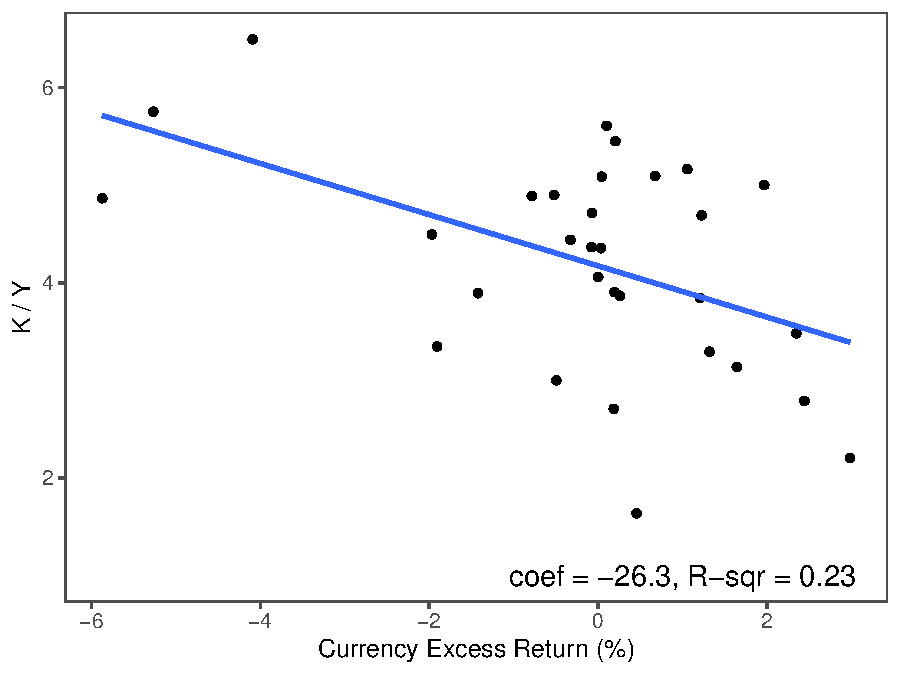
\includegraphics[width=0.7\linewidth]{Exhibits/Figure_KY_RX.pdf}
    \begin{minipage}[htp]{\textwidth}
    \scriptsize 
    \emph{Notes:} This figure shows the relationship between average currency excess returns and average capital-to-output ratios across currency regions. The coefficient is the slope of the line of best fit. The corresponding coefficient on a regression of capital-to-output ratios on interest rate differentials is -0.10.
    \end{minipage}
\end{figure}

Pushing beyond the aggregate data, Richers (2020) shows direct evidence of the link between  risk-free interest differentials and the cost of capital at the firm-level: Using data from the primary issuance of 100,000 corporate bonds of non-financial firms in 98 countries, he shows that differences in risk-free interest rates pass through almost one-for-one to firms' cost of borrowing. That is, firms borrowing in low-interest-rate currencies have cheaper access to credit than their counterparts who borrow in high-interest-rate currencies. These differences in bond-level yields cannot be explained with observable characteristics of firms issuing in different currencies, and even exist within firms who issue in multiple currencies within the same month. That is, the same firm issuing in Japanese yen and New Zealand dollars in the same month pays a several percentage point higher yield to maturity on the latter bond than the former bond. 

Consistent with these patterns, Richers (2020) also shows that firms which are headquartered in countries with higher interest rates produce more output per unit of capital installed, suggesting that these firms indeed operate at a higher marginal product of capital. 

Further adding evidence in favor of a risk-based interpretation of long-run differences in capital accumulation, \citet{DavidHenriksenSimonovska2014} show that although the returns to capital investment are higher in emerging market economies, these returns are also more correlated with the U.S. stock market. This pattern suggests emerging market economies are more exposed to systematic risk, which the authors interpret as long-run growth risk. Thus, capital investment in emerging markets should pay higher returns to compensate investors for this risk exposure. The authors go on to calibrate a model with recursive utility where countries are exposed long-run growth risk according to their empirical correlation with the U.S. stock market. Their model is able to quantitatively account for a significant portion of the variation in capital accumulation across countries.

This link between a country's risk characteristics and capital accumulation poses challenges and opportunities for several ongoing debates in the macroeconomics literature that have yet to be explored systematically and may prove fertile ground for future research. We outline each of these potential applications briefly below.

\subsection{The Lucas Paradox}

The variation in capital-to-output ratios across countries has itself of course been an active topic of research. In a seminal paper, \citet{Lucas1990} argued that large differences in capital accumulation implied large differences in the marginal product of capital (MPK). Given these large differences in MPK, \citet{Lucas1990} pointed out that not enough capital seemed to be flowing towards emerging market countries. This finding is known as the ``Lucas Paradox.''

The literature has debated various potential resolutions to the Lucas paradox and the associated lack in convergence in GDP per capita across countries (De Long, ...). These include heterogeneity
in the protection of property rights (Hall and Jones, 1997), taxation rates (Jorgenson,
1996), depreciation rates, the capital share of output (Karabarbounis and Neiman, 2014),
and distortions in the allocation of resources (Hsieh and Klenow, 2009). To our knowledge, neither the role of persistent differences in interest rates, nor the role of differences in currency or country risk have been systematically evaluated relative to this literature. In other words, one possible reason why we see persistent lack of convergence in capital-to-output ratios may simply be persistent differences in currency and country risk. 

\subsection{Measurement of MPK}

FIXMETH

Another potential resolution of the Lucas Paradox that has received considerable attention is that MPK may be poorly measured. The current allocation of capital across countries may indeed be efficient given the correct measurement of the expected returns to investment. For example, an influential paper by \citet{CaselliFeyrer2007} argued that land and other natural resources are crucial inputs to production in emerging market economies. Thus, the measure of MPK used in \citet{Lucas1990} conflates the returns to capital obtained through investment with the returns to natural resources. The authors augment the Cobb-Douglas production function to include natural resources, and measure the output share of natural resources using data from the World Bank. After accounting for the role of natural resources in production, the marginal product of capital obtained through investment is in fact roughly equal across countries. More recently however, \citet{Monge-Naranjoetal2019} provided a different methodology for estimating the output share of natural resources, and showed the expected return on capital investment still varied dramatically across countries after accounting for natural resources.

The common assumption in this literature, however, is that in the absence of these frictions, interest rates and the marginal product of capital should equalize across countries. 

Future work: Connection with currency risk, Ultimate reasons for exposure to common risks


\subsection{Currency Risk and Exchange Rate Regimes}

In addition to potentially shedding light on these long-standing puzzles in the literature, a recent paper by HMZ argues that the link between the stochastic properties of a country's real exchange rate and the level of capital accumulation also provides a new way of thinking about the costs and benefits of adopting different exchange rate regimes. 
The authors note that the pervasive practice among small and medium-sized economies to stabilize their exchange rate relative to the US dollar or the euro (Iletzki, Reinhart, and Rogoff) may be thought of as an attempt to make their currencies (and by extension their economies) a safer investment from the perspective of world investors. 

In their model, countries again differ in size and the domestic prices of traded goods are sticky in terms of the domestic currency, so that each country's central bank has some control of its country's real exchange rate. When a small country stabilizes its exchange rate relative to a larger target country its real exchange rate inherits the stochastic properties of that larger target currency, and thus becomes safer from the perspective of world investors. A safer currency in turns comes with a lower domestic risk-free rate, higher domestic capital accumulation and higher wages. That is, managing a country's exchange rate risk becomes a means of attracting international investment and raising the world-market value of domestic firms. 
In the absence of policy coordination, small countries then optimally choose to
stabilize their exchange rates relative to the currency of the largest economy in the world,
which endogenously emerges as the world's anchor currency." Larger economies instead
optimally choose to 
float their exchange rates, because currency interventions by larger countries are endogenously more expensive to maintain than those by smaller countries. The model therefore predicts an equilibrium pattern of exchange rate arrangements that is similar to the one in the data, where small countries below a certain size stabilize, intermediate-sized countries have looser stabilizations, and only the largest economies in the world float their currencies.

\section{Currency Risk on Corporate and Sovereign Balance Sheets}
Original sin literature WHAT ELSE EXISTS?

Need a benchmark model for currency composition of debt
\begin{enumerate}
\item \citet{Richers2019}
\item di Giovanni, Kalemli-Ozcan, Ulu, Baskaya (2019)
\item Boccola and Lorenzoni savers demanding FC deposits to insure agains tdepreciation risk
\item Salomao and Varela
\item Du and Schreger Firms loading up on foreign currency debt to borrow at lower interest rates increases sovereign default risk.
\item Corlin du schreger portofolio choice model JF
\item Ottenello and Perez - AEJ Macro
\end{enumerate} 
Macroproudential

Balance sheets and exchange rate policy Cespedes Chang Velasco 


\section{The Dynamics of Currency Risk}


Up until this point, we have focused primarily on the cross-sectional implications of currency risk premia, which has also been the focus of the most recent literature. A natural extension of this discussion is to understand the effects of risk premia for currency return dynamics and capital accumulation. As stated in Section XX, much of the early work on currency risk began as an attempt to understand the forward premium puzzle --- The finding that, on average, high-interest-rate currencies do not depreciate enough to wipe out any differences in interest rates. In addition, many studies have highlighted an apparent disconnect between macroeconomic variables and variation in exchange rates \citep{MeeseRogoff1983,BackusSmith1993}, and that exchange rates appear surprisingly volatile compared aggregate consumption growth. In response to these empirical facts, a large theoretical literature has argued that time variation in currency risk premia may be able to jointly rationalize these facts \citep{Fama1984,Backusetal2001}.

One strategy for introducing large amounts of time variation of currency risk premia involves using more complicated investor preferences from the asset pricing literature that have helped resolve other asset pricing anomalies. \citet{Verdelhan2010} proposed a model in which representative investors of each country exhibit preferences for an exogenously specified ``habit'' level of consumption. As a country's consumption approaches its habit level, the domestic investor becomes much more risk-averse. This increase in risk-aversion lowers the domestic interest rate while also increasing the currency's risk premium. In the extreme, this mechanism can even rationalize a situation where investors expect currencies that have unusually high interest rates to appreciate (the ``Fama conditions'').  Building on this intuition, \citet{Heyerdahl-Larsen2011} shows that adding ``deep habits'' -- habits for specific goods within the consumption basket -- allows the model to match the term structure of bond yields as well the dynamics of exchange rates. Moreover, \citet{Stathopoulos2017} shows that one can also rationalize the low volatility of real exchange rates and the disconnect between exchange rates and consumption by adding consumption home bias (in addition to habit preferences). 

An alternative assumption is to endow investors with Epstein-Zin utility functions and allow for long-run risks. Within these models, the covariance structure of long-term consumption growth shocks strongly impacts exchange rates today. \citet{ColacitoCroce2011} show that a model with highly correlated long-term growth shocks can produce a low correlation in consumption across countries along with a realistic volatility of exchange rates. \citet{BansalShaliastovich2012} and \citet{ColacitoCroce2013} further show that long-run news shocks partnered with a high enough intertemporal elasticity of substitution also produces the comovement of interest rates and currency risk premia required to explain the forward premium puzzle. 

\begin{enumerate}
    \item \citet{GourioSiemerVerdelhan2013}
    \item \citet{FarhiGabaix2016}
    \item Guo (2010) Du (2013) Martin (2013)
    \item \citet{Backusetal2001}
\end{enumerate}

 



In light of our discussion of above, there are at least three avenues for further developing this dynamic literature. First, there is a clear need for synthesis. None of the models that match the cross-section have much to say about dynamics, and vice versa. Given that many of the dynamic models have within them various approaches to rationalize large risk premia, there is also reason to hope that some of these tools may be effective in addressing the (quantitative) interest differential puzzle as we have stated it in section XX above. 

Second, although the various theories of the dynamics of currency risk provide ways to rationalize the stochastic behavior of interest rates and exchange rates, it is unclear whether these models can also explain the dynamics of capital accumulation. One paper that makes some progress in this direction is \citet{ColacitoCroceHoHoward2018}. Building on \citet{ColacitoCroce2011, ColacitoCroce2013}, \citet{ColacitoCroceHoHoward2018} endows investors with Epstein-Zin utility and allows for both short-term and long-term shocks to productivity. The authors show that an appropriate calibration of the long-term productivity shock process allows the model to explain
the response of capital flows to productivity shocks between two representative developed economies. However, there is clearly more work to be done, particularly given that not a single quantitative paper attempts to account for the link between interest rate differentials and capital-to-output ratios in the cross-section, let alone the dynamic responses of capital flows to changes in exchange rate policy or other shocks.

Third, if we really believe that currency and country risks vary over time, then it should be possible to measure these time-varying perceptions of risk. Two promising 



\subsection{Measurement of risk FIXMETH}
Maybe measurement of risk - implied vol - commercial indices - newspapers - conference call transcripts


\section{Conclusion}


***** Probably won't use ******************************


\section*{Capital flows and the allocation puzzle}
Capital flows run counter to neo-classical model:
\begin{enumerate}
\item \citet{GourinchasJeanne2013}
\item[-] Current explanations:
\item Differences in financial development (Ju and Wei, 2006;
  Caballero, Farhi and Gouinchas, 2008; Mendoza, Quadrini and
  Rios-Rull, 2009)
\item Differences in factor utilization (Jin, 2012)
\item Differences in contracting frictions (Aguiar and Amador, 2010)
\end{enumerate}


\subsection{Unsorted}
\begin{enumerate}
\item Gourinchas and Rey (2007)
\item Burnside, Eichenbaum, Kleshchelski and Rebelo (2011)
\end{enumerate}



\subsection{Sidebars and Margin Notes}
% Margin Note
\begin{marginnote}[]
  \entry{Term A}{definition} \entry{Term B}{definition} 
\end{marginnote}


% Summary Points
\begin{summary}[SUMMARY POINTS]
  \begin{enumerate}
  \item Summary point 1. These should be full sentences.

  \end{enumerate}
\end{summary}

% Future Issues
\begin{issues}[FUTURE ISSUES]
  \begin{enumerate}
  \item Future issue 1. These should be full sentences.
  \end{enumerate}
\end{issues}

\newpage

\setstretch{1}

\bibliographystyle{chicago} \bibliography{ARE}

\clearpage


\appendix

\begin{center}
  {\Huge\bf Appendix}\\
  {\large\bf -For online publication only-}
\end{center}

\section{Derivation of Equation \ref{eq_UIP_RF} \label{Appendix_ReducedFormResults}}

The country $n$ risk-free bond pays off $P_n$ units of the traded good at maturity. We derive the value of the risk-free bond, $V_n$, by applying the asset pricing equation to the bond payoff: 
\begin{equation*}
  V_n = \mathbb{E}\left[M_{T} P_n
  \right],
\end{equation*}
where $M_{T}$ denotes the stochastic discount factor. The country $n$ risk-free rate (in levels), $R^f_n$, is the inverse of the price of the risk-free bond:
\begin{equation*}
  R^f_n = \frac{1}{V_n}.
\end{equation*}
Putting the previous two equations together yields the following relationship:
\begin{equation*}
  \mathbb{E}\left[ M_T P_n \right] R^f_n = 1.
\end{equation*}
As a result, the risk-free rates of countries $f$ and $h$ are related as follows:
\begin{equation*}
  \mathbb{E}\left[M_T P_f \right] R^f_f 
  = \mathbb{E}\left[M_T P_h \right] R^f_h = 1
\end{equation*} 
If the stochastic discount factor and prices are log-normal, we can perform the following calculations:
\begin{align*}
  & \mathbb{E}\left[M_{T} P_f \right] R^f_f
    = \mathbb{E}\left[M_{T} P_h \right] R^f_h \\
  \Leftrightarrow\quad
  & \mathbb{E}\left[\exp\left[ m_T + p_f + r^f_f \right]\right]
    = \mathbb{E}\left[\exp\left[ m_T + p_h + r^f_h \right]\right] \\
  \Leftrightarrow\quad
  & \mathbb{E}\left[m_T + p_f\right] + \frac{1}{2}\text{var}\left(m_T\right) +      \frac{1}{2}\text{var}\left(p_f\right) + \text{cov}\left(m_{T}, p_f\right) + r^f_f \\
  & = \mathbb{E}\left[m_{T}+ p_h\right] + \frac{1}{2}\text{var}\left(m_{T}\right) + \frac{1}{2}\text{var}\left(p_h\right) + \text{cov}\left(m_T, p_h\right) + r^f_h,
\end{align*}
We cancel out $\text{var}\left( m_T \right)$ from both sides of the previous equation.
\begin{align*}
  & \mathbb{E}\left[p_f\right]+\frac{1}{2}\text{var}\left(p_f\right) + \text{cov}\left(m_T, p_f\right) + r^f_f = \mathbb{E}\left[p_h\right]+\frac{1}{2}\text{var}\left(p_h\right)+\text{cov}\left(m_T,p_h\right) + r^f_h
  \\      \Leftrightarrow \quad
  & r^f_f+\mathbb{E}\left[p_f-p_h\right]+\frac{1}{2}\text{var}\left(p_f\right)-\frac{1}{2}\text{var}\left(p_h\right)-r^f_h = -\text{cov}\left(m_T,p_f-p_h\right)\\   
  \Leftrightarrow\quad
  &r^f_f+\log\left(\mathbb{E}\left[P_f\right]/\mathbb{E}\left[P_h\right]\right)-r^f_h = -\text{cov}\left(m_T,p_f-p_h\right)
\end{align*}
We define
$\Delta\mathbb{E}\left[s_{f,h}\right]
=\log\left(\mathbb{E}\left[P_f\right]/\mathbb{E}\left[P_h\right]\right).$
With this definition:
\begin{equation*} 
  r^f_f+\Delta\mathbb{E}\left[s_{f,h}\right]-r^f_h = -\text{cov}\left(m_T,p_f-p_h\right). 
\end{equation*}

\section{Derivation of Equation \ref{eq_BFT} \label{Appendix_BFT}}

Letting $M_n$ denote the stochastic discount factor measured in units of the consumption bundle specific to country $n$ and assuming no arbitrage, we know the risk-free rate in country $n$ satisfies:
\begin{equation*}
    R^f_n = \frac{1}{\mathbb{E} \left[ M_n\right] }
\end{equation*}
If we further assume $M_n$ is log-normally distributed, then
\begin{eqnarray*}
r^f_n &=&-\log \left( E\left[ M_n \right] \right)  \\
&=&-\left( E\left[ m_n \right] +\frac{1}{2}\text{var}\left[ m_n \right] \right) 
\end{eqnarray*}
Next, take the difference between the risk-free rates of countries $f$ and $h$:
\begin{eqnarray*}
r^f_f - r^f_h  
&=& -\left( \mathbb{E} \left[ m_f \right] +\frac{1}{2}\text{var}\left[ m_f \right] \right) 
+ \left( \mathbb{E}\left[ m_h \right] +\frac{1}{2}\text{var}\left[ m_h \right] \right)  \\
r^f_f-r^f_h + \mathbb{E} \left[ m_f - m_h \right] 
&=& \frac{1}{2}\left( \text{var}\left[ m_h \right] - \text{var}\left[ m_f \right] \right) 
\end{eqnarray*}
Finally, when financial markets are complete, $\Delta s_{f, h} = m_f - m_h$. Thus
\begin{eqnarray*}
r^f_f + \mathbb{E} \Delta s_{f, h} - r^f_h 
&=& \frac{1}{2}\left( \text{var}\left[ m_h \right] - \text{var}\left[ m_f \right] \right)
\end{eqnarray*}
    

\end{document}